%% 
%% Libro en español
%% Pantilla Latex para estructura de un libro en español
%% Autor: Dario A. Palminio
%% Colaborador: David Alderete
%% LaTeX versión: 2.0
%% Sistema operativo: Ubuntu
%% Editor usado: LaTeXila 2.4.0
%% 

\documentclass[a4paper,11pt]{book}

% Imports
\usepackage[T1]{fontenc}
\usepackage[utf8]{inputenc} %% file charset=utf-8
\usepackage{lmodern}
\usepackage{graphicx}

% Image location
\graphicspath{ {images/} }

% Rename names to spanish language
\renewcommand{\contentsname}{Índice}
\renewcommand{\chaptername}{Capítulo}
\renewcommand{\bibname}{Bibliografía} % Bibliography in spanish
\renewcommand{\figurename}{Figura}

\begin{document}

% General structure
%%%%%%%%%%%%%%%%%%%%%%%%%%%%%%%%%%%%%%%%%%%%%%%%%%%%%%%%%%%%%\
%%%% Author & title page info

% Book's title and subtitle
\title{\Huge 
    \textbf{Titulo}  \\ 
    \huge Subtitulo
    }

% Book's author
\author{Dario Palminio, David Alderete}

% Book's date
\date{2015} 

\maketitle


%% 

\tableofcontents
\newpage
\listoffigures
%%\newpage
%%\listoftables

%% This is an example first chapter. 

\chapter{Introducción}

Texto del Capítulo 1 \cite{Einstein-2008}

\begin{figure}[h]
  
\includegraphics{image_001}
  \caption{Ejemplo de imagen}
  \centering
  \label{fig:ejemplo} %\ref{fig:ejemplo}
\end{figure}

\section{Título de la sección primera}

Texto de la sección 1 


\subsection{Título de la sub-sección primera}

Texto de la sub-sección 1

%% Chapter: Sistemas

\chapter{Sistema General}

Texto del Capítulo 2

\section{Introducción al sistemismo}
\section{Noción de Agregado}
\section{Noción de Sistema}
\subsection{Estructura}
\subsection{Organización}
\subsection{Evolución}
\section{Noción de niveles}
\section{Sistemización}
\subsection{Sistema mecánico}
\subsection{Sistema Orgánico}
\subsection{Sistemisidad}
\subsection{Acoplamiento}
\subsection{Cohesión}

\section{Noción de  emergentismo}
\subsection{El concepto de emergencia}
\subsubsection{Emergencia en niveles}
\subsubsection{Definición de emergencia}
\subsubsection{Las cosas que emergen}

\subsection{Características constitutivas}
\subsection{Emergencia de Sistemas}
\subsection{Inteligencia de enjambre}
\subsubsection{Inteligencia de la multitud}

\section{Cibernética}

%% Chapter: Modelado de Sistemas

\chapter{Modelado de Sistemas}

El Modelado de Sistemas es una actividad esencial de Ingeniería de Sistemas, de sistemistas y de cualquier pensador sistémico. Pues, se hacen modelos como simplificación abstracta de la realidad \cite{Meadows-2009} que forma una representación del sistema real \cite{Fiuba-2005} o sistema origen a estudiar o sistema a diseñar.

\section{Sistema de modelado}

Para entender la realidad se hace necesario percibirla y modelarla de algún modo. En este proceso existe un orden real de las cosas y un orden percibido y reflejado en un modelo hecho por alguien, un observador o modelizador (Modeler/Observer). Como dijo Capra “toda la percepción de un modelo es, de alguna manera, la percepción de algún orden” \cite{Fritjof-Capra-1975} y la percepción de un orden es hecha por alguien. Un principio cibérnetico dice que todo fenómeno observado es observado por alguien (Heinz Von Foerster, 1979) que en otras palabras quiere decir que “todo conocer depende de la estructura del que conoce” \cite{Maturana-1984}. Por este motivo, el proceso de modelado constituye un sistema de modelado en el que existe un observador modelizador como un elemento principal del mismo. Pero, como interviene un observador, entonces la observación y su modelado se torna subjetiva. Para hacer que el modelo sea más objetivo y tenga alguna consistencia con la realidad modelada son necesarios conocimientos científico-técnicos que nos permitan cierta fiabilidad y herramientas conceptuales y físicas para realizar dicha tarea bajo cierta estandarización. Los conocimientos científico-técnicos empleados como herramienta conceptual para modelar en un marco de trabajo sistémico pertenecen principalmente a la Teoría General de Sistemas o SGT (General System) \cite{Sarabia-1995}. Y las herramientas conceptuales para modelar (Tools) pueden ser herramientas útiles para aplicar SGT en el proceso de modelado, como pueden ser las herramientas de diagramación, la matemática y la lógica. A este "proceso de modelización" (Modeling) también se lo puede llamar "Sistemografear" \cite{Le-Moigne-1994} y tiene como entrada principal la persepción y medida del objeto estudiado o "sistema real" (Real System) y como salida principal el sistema modelo (Model System) o sistema conjunto de modelos (ver figura \ref{fig:ModelingSystem}).

\begin{figure}[h]
  \centering
  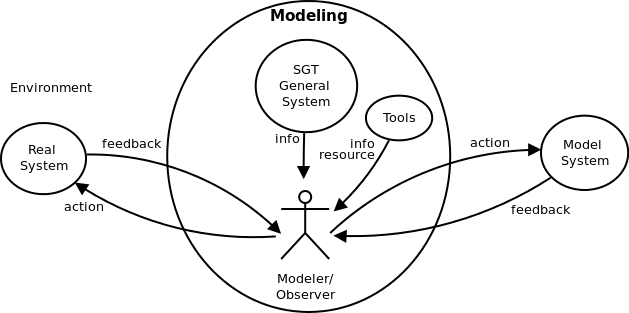
\includegraphics[scale=0.5]{ModelingSystem}
  \caption{Sistema de modelado}
  \centering
  \label{fig:ModelingSystem} %\ref{fig:ModelingSystem}
\end{figure}

Hay que tener en cuenta que este proceso es dinámico y mientras se desarrolla el mismo, el modelador, a la vez que recibe una retroalimentación del sistema modelo, puede estar modificando al sistema real, que a su vez lo lleva a modificar también al sistema modelo. Esta idea nos lleva a pensar a un modelo sistémico como un flujo de información procesado por el modelizador usando al Sistema General SGT \cite{Sarabia-1995}.

\section{Herramientas conceptuales de modelado}

Hay diferentes maneras de plasmar un modelo fuera de nuestras mentes. Entre las más usadas estan la representación gráfica con diagramación, la modelización matemática y la modelización informática. Estas maneras son herramientas usadas por un sistemista para poder modelar. Las herramientas conceptuales de modelado sirven, entre otras cosas, para construir modelos de caja negra sin los detalles atinentes a la composición material de los sistemas concretos modelados \cite{Bunge-1979}. La teoría sistémica SGT sirve como principal herramienta conceptual que brinda las teorías, conceptos y formas de enfoque para poder analizar la porsión de mundo a modelar por el sistemista modelizador. Si bien todo el conocimiento científico funciona como herramienta conceptual, al sistemista generalmente no le interesa incorporar leyes específicas de las ciencias de nivel inferior de realidad (como la física y la química) sino, más bien, le interesa aplicar leyes generales transversales a diferentes disciplinas. Por este motivo la teoría sistémica sirve a este propósito, como herramienta generalista para el trabajo multidisciplanrio de analisis sistémico.

\subsection{Herramientas conceptuales de Diagramado}

La gráfica o la diagramación es una de las herramientas más usadas en análisis de sistemas. La diagramación es una herramienta metodológica fundamental del proceder empírico en estudio y diseño de sistemas y arquitecturas. Los diagramas habitualmente sirven para modelar la realidad con un lenguaje simbólico gráfico y su utilidad es la siguiente:

\begin{itemize}

\item \textbf{Persepción visual:} la representación visual sirve para comprender y recordar mejor. La visión es, por lejos, nuestro sentido más dominante. Por lo general aprendemos y recordamos mejor a través de imágenes, no a través de la expresión oral o escrita. Si escuchamos un fragmento de información y tres días después recordamos el 10 por ciento de él, agregando una imagen recordaremos aproximadamente un 55 por ciento más \cite{John-Medina-2008}. Este es un buen argumento para trabajar con irradiadores visuales de información y también para usar diagramas para comprender sistemas que también pueden funcionar como irradiadores visuales de información.

\item \textbf{Comprención sistémica:} el análisis de sistemas se basa en el análisis de organización y la organización es mejor comprendida usando simbología visual más que con solo simbología matemática y lenguaje escrito. En principio por lo antes mencionado y luego por razones sistémicas. Partiendo de la premisa de que "una forma de lenguaje presupone una forma de ver el mundo" \cite{David-Bohm-2008}, se puede decir que un diagrama sistémico conforma un lenguaje simbólico que es una manera de formarse una idea de una porsión de mundo muy distinta a la usada con el lenguaje corriente. Por ejemplo el lenguaje corriente escrito (como el español o el inglés) presupone, hasta cierto punto, una forma fragmentaria y secuencial de ver el mundo. En cambio un diagrama sistémico puede colaborar en brindar una forma de ver totalizadora no fragmentaria y no secuencial, donde el todo diagramado es un movimiento global donde cada cosa es una abstracción relativamente invariante de el movimiento en un contexto de totalidad.

\item \textbf{Comunicación de ideas:} Como dijera Albert Einstein: "si no puedes explicarlo simple, no lo entiendes lo suficientemente bien"; y la diagramación sirve para hacer más simple una explicación de un sistema complejo. En este sentido sirve al trabajo cooperativo de diseño y creación y a la comunicación de los resultados del diseño. Es útil al trabajo cooperativo de diseño debido a que nos permite debatir, representar en gráficos y tener "referentes concretos" compartidos de los conceptos que conversamos. El principal valor de los diagramas se da en el debate, porque mientras diagramamos modelamos para mantener una conversación; pues, el valor principal es la conversación y la comprensión compartida al crear el modelo; su visualización como un diagrama fácil de ver es importante para hacer concretas y sin ambigüedades a las ideas que tenemos, los modelos mentales de las personas, porque las palabras solas pueden ser borrosas y mal entendidas \cite{Larman-Vodde-2008}. De este modo, un diagrama sistémico o arquitectónico sirve a los propósitos de Ingeniería de Sistemas y a la Arquitectura para comunicación y medio de educación. Y tomando el argumentos previos podemos decir que: comunicar ideas en forma visual es más efectivo.

\item \textbf{Guía de desarrollo:} así como la arquitectura sirve para ser una guía en la construcción de obras y la arquitectura de softwaer como guía en la programación de software, el diagramado con sus diagramas sistémicos sirve como guía al diseño arquitectónico y de sistemas, por lo que, en consecuencia, sirve al desarrollo de sistemas.

\end{itemize}

A continuación se listan las herramientas principales más conocidas:

\begin{table}[h]
\centering
\caption{Herramientas conceptuales de Diagramado}
\label{Herramientas-conceptuales-de-Diagramado}
\begin{tabular}{|l|l|}
\hline
Acrónimo & Significado en inglés                         \\ \hline
Graph    & Graph Diagram                                 \\ \hline
ADL      & Architecture Description Language             \\ \hline
BPMN     & Business Process Modeling Notation            \\ \hline
CD       & Conceptual Diagram or ConceptDraw             \\ \hline
CLD      & Causal Loop Diagram                           \\ \hline
ERD      & Entity Relationship Diagram                   \\ \hline
FC       & Flow Charts (for control flow)                \\ \hline
DFD      & Data Flow Diagram                             \\ \hline
MMD      & Map Mind Diagram                              \\ \hline
SC       & Structure Chart                               \\ \hline
SFD      & Stock and Flow Diagrams                       \\ \hline
SSADM    & Structured Systems Analysis and Design Method \\ \hline
UML      & Unified Modeling Language                     \\ \hline
\end{tabular}
\end{table}

\subsubsection{Graph, Diagrama de Grafos}

Un grafo es un conjunto de objetos llamados nodos (vértices) unidos por enlaces llamados aristas (arcos). Un grafo es la manera más simple de representar un sistema en forma gráfica ya que los nodos pueden representar a los componentes del sistema y las aristas a las relaciones entre los componentes. El diagrama de grafos es la base de muchos otros diagramas como: diagramas conceptuales, grafos Pert y diagramas de Gantt.

\begin{figure}[h]
  \centering
  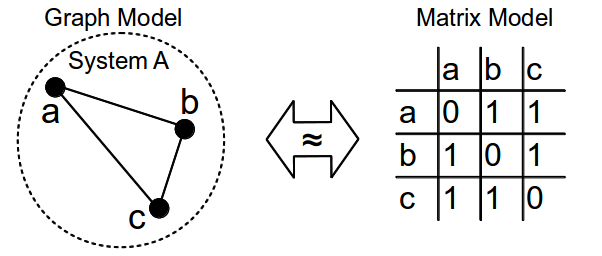
\includegraphics[scale=0.5]{GraphModelBasic}
  \caption{Ejemplo de Diagrama de Grafos simple}
  \centering
  \label{fig:GraphModelBasic} %\ref{fig:GraphModelBasic}
\end{figure}


\subsubsection{ADL}

\subsubsection{BPMN}

\subsubsection{CD}

\subsubsection{CLD, Diagrama de Lazos Causales}
El Diagrama de Lazos Causales, CLD o Causal Loop Diagram...

\begin{figure}[h]
  \centering
  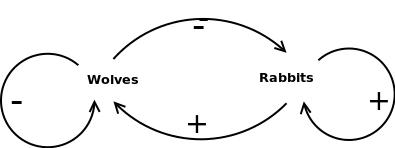
\includegraphics[scale=0.5]{CausalLoopDiagramWolvesAndRabbitsExample}
  \caption{Ejemplo de un Diagrama de Lazos Causales}
  \centering
  \label{fig:v} %\ref{fig:CausalLoopDiagramWolvesAndRabbitsExample}
\end{figure}

\subsubsection{ERD}

\subsubsection{FC, Gráfico de Flujo}

El Diagrama de Flujo o Gráfico de flujo (FC o "Flow Charts") es usado para diagramar flujos de control.

\subsubsection{DFD, Diagrama de Flujo de Datos}

El Diagrama de Flujo de Datos o DFD fue introducido y popularizado en 1970 para el análisis y diseño estructurado \cite{Gane-Sarson-1979} para diagramar procesos de sistemas. Un DFD muestra el flujo de datos dentro del sistema desde entidades externas, mostrando cómo los datos fluyen entre diferentes procesos y qué almacenes intervienen para que los datos sean guardados y recuperados \cite{Scott-Ambler-2004}. Los modelos DFD muestran una perspectiva funcional de un sistema donde cada transformación o proceso representa una función que el sistema hace en su procesamiento de entradas en salidas \cite{Sommerville-2006}.\newline
Para este tipo de diagramas hay dos estándares de notaciones: la notación DeMarco-Yourdon (DeMarco, Yourdon y Constantine 1979 \cite{Dixit-2007}) y la notación Gane-Sarson.\newline
\newline

En este tipo de diagramas hay solo cuatro elementos \cite{Dixit-2007}:
\begin{itemize}
\item \textbf{Entidad externa:} las entidades externas son fuentes de recursos de datos externos al sistema, aunque también podrían ser de materia, energía o información. Se los suele identificar con sustantivos que son el nombre de la entidad. Por ejemplo un proveedor del sistema, un cliente, etcétera.

\item \textbf{Proceso:} son los subsistemas o procesos del sistema. Un proceso es como una caja negra cuya estructura interna no se muestra y que posee entradas y salidas, considerándose a las mismas como flujos. Un proceso es una actividad de procesamiento de datos, pero también podría serlo de materia, energía o información. Un proceso también puede verse como un sistema o subsistema componente de otro, ya que es una estructura funcionando en el tiempo. En Teoría General de Sistemas se tiene una persepción dinámica de la realidad, donde los sistemas son considerados procesos \cite{Sarabia-1995}. A los procesos se los suele identificar con nombres descriptivos que son verbos, verbos en infinitivo, verbos con sufijo "-ción/-sión" o nombre de actividad que se asocia a una acción o proceso.

\item \textbf{Flujo de dato:} también están los flujos de datos electrónicos o físicos. Un flujo es un fenómeno identificable por el cual se reconoce la interacción entre procesos como transferencia, transacción o suceso. Los flujos son las relaciones en un sistema. Habitualmente se asocia al flujo con transferencia de datos, pero también puede ser de materia o energía. Se los suele identificar con sustantivos que son el nombre del objeto o suceso que es transferido en el flujo.

\item \textbf{Almacen:} un almacen es una entidad para guardar y recuperar información, materia o energía. Esta entidad es un componente de almacenamiento del sistema. Se los suele identificar con sustantivos que son el nombre de la entidad de almacenado o almecen de los objetos del flujo. Por ejemplo un almacén puede ser un depósito, una librería, etcétera.

\end{itemize}

\textbf{DFD con notación Gane-Sarson}

En notación Gane-Sarson las entidades externas se representan con rectángulos o cuadrados, los procesos se representa con rectángulos redondeados, los flujos con flechas y los almacenes con rectángulos abiertos. A continuación se puede ver un ejemplo (ver figura \ref{fig:DFDGaneSarsonNotation}):\newline
\newline

\begin{figure}[h]
  \centering
  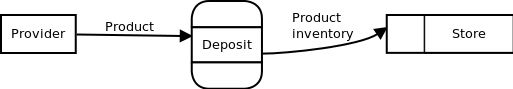
\includegraphics[scale=0.5]{DFDGaneSarsonNotation}
  \caption{DFD Notación Gane-Sarson \cite{Gane-Sarson-1979}}
  \centering
  \label{fig:DFDGaneSarsonNotation} %\ref{fig:DFDGaneSarsonNotation}
\end{figure}

\textbf{Ejemplo de DFD con notación DeMarco-Yourdon}

En notación DeMarco-Yourdon las entidades externas se representan con rectángulos o cuadrados, los procesos se representa con círculos o elipses y los almacenes con rectángulos sin líneas laterales. Por practicidad se puede implementar con un rectángulo con algún distintivo, siempre cuando se aclare que la notación representa un almacen de datos. A continuación se puede ver un ejemplo (ver figura \ref{fig:DFDDeMarcoYourdonNotation}):\newline
\newline

\begin{figure}[h]
  \centering
  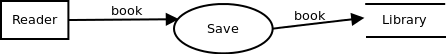
\includegraphics[scale=0.5]{DFDDeMarcoYourdonNotation}
  \caption{Ejemplo de DFD Notación DeMarco-Yourdon \cite{Dixit-2007}}
  \centering
  \label{fig:DFDDeMarcoYourdonNotation} %\ref{fig:DFDDeMarcoYourdonNotation}
\end{figure}


\subsubsection{MMD}

\subsubsection{SC}

\subsubsection{SFD}

\subsubsection{SSADM}

\subsubsection{UML}

\section{Modelos de un sistema general}
\section{Sistema general de modelado}
\section{Modelo de sistemas generales básicos}
\subsection{Sistemas termodinámicos}
\subsection{Sistema aislado en equilibrio termodinámico}
\subsection{Sistema aislado tendiente al equilibrio}
\subsection{Sistema abierto en equilibrio estacionario}
\subsection{Sistema Sistemas en Equilibrio Dinámico}
\subsection{Sistemas Sostenibles y Sostenibilidad}
\subsection{Sistema Mínimo de Vida}
\subsection{Sistema Agente}
\subsection{Sistema Autopoiético Mínimo}
\section{Modelos de Sistemas Cibernético}

\subsection{Sistema Cibernético General}
\subsubsection{Ejemplo 1: Sistema regulador de tanque de agua}
\subsubsection{Ejemplo 2: Sistema regulador de Watt}
\subsubsection{Sistema Cibernético Auto-Aprendiente}
\subsubsection{Sistema Cibernético Auto-Organizado}
\subsubsection{Sistema Cibernético Auto-Aprendiz y Auto-Organizado}

\subsection{Modelos de organizaciones}
\subsubsection{Viable System Model}

%% This is an example first chapter. 

\chapter{Ingeniería}

Texto del Capítulo 2

\section{Título de la sección primera}

Texto de la sección 1


\subsection{Título de la sub-sección primera}

Texto de la sub-sección 1


%% This is an example first chapter. 

\chapter{Sistemas Software}

Texto del Capítulo 2

\section{Título de la sección primera}

Texto de la sección 1


\subsection{Título de la sub-sección primera}

Texto de la sub-sección 1


%% This is an example first chapter. 

\chapter{Sistema de Ideas}

Texto del Capítulo 2

\section{Principios}

Texto de la sección 1


\subsection{Título de la sub-sección primera}

Texto de la sub-sección 1

\section{Paradigmas}

Texto de la sección 2

\section{Filosofías}

Texto de la sección 3

%% This is an example first chapter. 

\chapter{Metodologías}

Texto del Capítulo 2

\section{Título de la sección primera}

Texto de la sección 1


\subsection{Título de la sub-sección primera}

Texto de la sub-sección 1


%% Chapter. 

\chapter{Arquitectura}

Generalidades, Arquitectura de Sistemas y Arquitectura de Software

% Section
\section{Generalidades}

Texto de la sección Generalidades


\subsection{Título de la sub-sección primera}

Texto de la sub-sección 1


% Section
\section{Arquitectura de Sistemas}

Texto de la sección Arquitectura de Sistemas


\subsection{Título de la sub-sección primera}

Texto de la sub-sección 1


% Section
\section{Arquitectura de Software}

Texto de la sección Arquitectura de Software


\subsection{Título de la sub-sección primera}

Texto de la sub-sección 1


\chapter{Glosario y Acrónimos}

\begin{table}[h]
\begin{tabular}{lllll}
\cline{1-2}
\multicolumn{1}{|l|}{Nombre} & \multicolumn{1}{l|}{Detalle}                              &  &  &  \\ \cline{1-2}
\multicolumn{1}{|l|}{SAD}  & \multicolumn{1}{l|}{Software Architecture Documentation} &  &  &  \\ \cline{1-2}
\multicolumn{1}{|l|}{SW}   & \multicolumn{1}{l|}{Software}                            &  &  &  \\ \cline{1-2}
                           &                                                          &  &  & 
\end{tabular}
\end{table}


% Bibliography
\bibliographystyle{apalike}
\bibliography{content/bibliography_list}

\end{document}
